% Created by tikzDevice version 0.6.2-92-0ad2792 on 2013-04-07 18:07:49
% !TEX encoding = UTF-8 Unicode
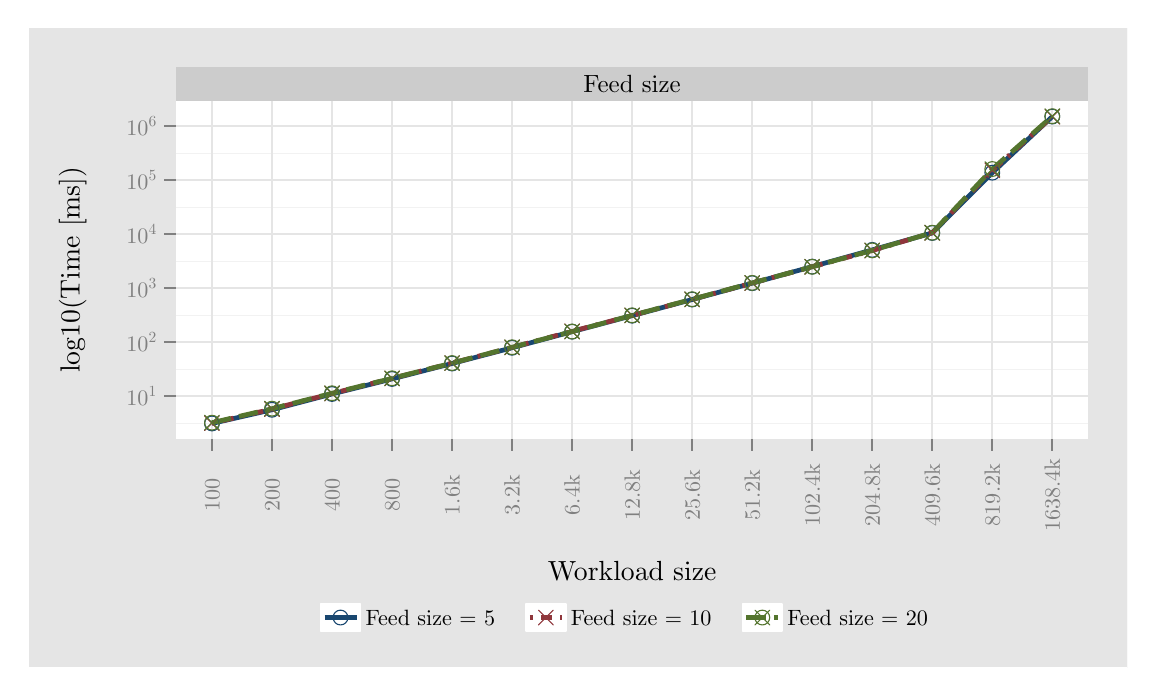
\begin{tikzpicture}[x=1pt,y=1pt]
\definecolor[named]{fillColor}{rgb}{1.00,1.00,1.00}
\path[use as bounding box,fill=fillColor,fill opacity=0.00] (0,0) rectangle (397.48,231.26);
\begin{scope}
\path[clip] (  0.00,  0.00) rectangle (397.48,231.26);
\definecolor[named]{drawColor}{rgb}{1.00,1.00,1.00}
\definecolor[named]{fillColor}{rgb}{0.90,0.90,0.90}

\path[draw=drawColor,line width= 0.6pt,line join=round,line cap=round,fill=fillColor] (  0.00,  0.00) rectangle (397.48,231.26);
\end{scope}
\begin{scope}
\path[clip] ( 53.58, 82.69) rectangle (383.26,204.82);
\definecolor[named]{fillColor}{rgb}{1.00,1.00,1.00}

\path[fill=fillColor] ( 53.58, 82.69) rectangle (383.26,204.82);
\definecolor[named]{drawColor}{rgb}{0.95,0.95,0.95}

\path[draw=drawColor,line width= 0.3pt,line join=round] ( 53.58, 88.33) --
	(383.26, 88.33);

\path[draw=drawColor,line width= 0.3pt,line join=round] ( 53.58,107.85) --
	(383.26,107.85);

\path[draw=drawColor,line width= 0.3pt,line join=round] ( 53.58,127.36) --
	(383.26,127.36);

\path[draw=drawColor,line width= 0.3pt,line join=round] ( 53.58,146.88) --
	(383.26,146.88);

\path[draw=drawColor,line width= 0.3pt,line join=round] ( 53.58,166.40) --
	(383.26,166.40);

\path[draw=drawColor,line width= 0.3pt,line join=round] ( 53.58,185.92) --
	(383.26,185.92);
\definecolor[named]{drawColor}{rgb}{0.90,0.90,0.90}

\path[draw=drawColor,line width= 0.6pt,line join=round] ( 53.58, 98.09) --
	(383.26, 98.09);

\path[draw=drawColor,line width= 0.6pt,line join=round] ( 53.58,117.60) --
	(383.26,117.60);

\path[draw=drawColor,line width= 0.6pt,line join=round] ( 53.58,137.12) --
	(383.26,137.12);

\path[draw=drawColor,line width= 0.6pt,line join=round] ( 53.58,156.64) --
	(383.26,156.64);

\path[draw=drawColor,line width= 0.6pt,line join=round] ( 53.58,176.16) --
	(383.26,176.16);

\path[draw=drawColor,line width= 0.6pt,line join=round] ( 53.58,195.68) --
	(383.26,195.68);

\path[draw=drawColor,line width= 0.6pt,line join=round] ( 66.60, 82.69) --
	( 66.60,204.82);

\path[draw=drawColor,line width= 0.6pt,line join=round] ( 88.29, 82.69) --
	( 88.29,204.82);

\path[draw=drawColor,line width= 0.6pt,line join=round] (109.97, 82.69) --
	(109.97,204.82);

\path[draw=drawColor,line width= 0.6pt,line join=round] (131.66, 82.69) --
	(131.66,204.82);

\path[draw=drawColor,line width= 0.6pt,line join=round] (153.35, 82.69) --
	(153.35,204.82);

\path[draw=drawColor,line width= 0.6pt,line join=round] (175.04, 82.69) --
	(175.04,204.82);

\path[draw=drawColor,line width= 0.6pt,line join=round] (196.73, 82.69) --
	(196.73,204.82);

\path[draw=drawColor,line width= 0.6pt,line join=round] (218.42, 82.69) --
	(218.42,204.82);

\path[draw=drawColor,line width= 0.6pt,line join=round] (240.11, 82.69) --
	(240.11,204.82);

\path[draw=drawColor,line width= 0.6pt,line join=round] (261.80, 82.69) --
	(261.80,204.82);

\path[draw=drawColor,line width= 0.6pt,line join=round] (283.49, 82.69) --
	(283.49,204.82);

\path[draw=drawColor,line width= 0.6pt,line join=round] (305.18, 82.69) --
	(305.18,204.82);

\path[draw=drawColor,line width= 0.6pt,line join=round] (326.87, 82.69) --
	(326.87,204.82);

\path[draw=drawColor,line width= 0.6pt,line join=round] (348.56, 82.69) --
	(348.56,204.82);

\path[draw=drawColor,line width= 0.6pt,line join=round] (370.25, 82.69) --
	(370.25,204.82);
\definecolor[named]{drawColor}{rgb}{0.10,0.28,0.44}

\path[draw=drawColor,line width= 1.7pt,line join=round] ( 66.60, 88.24) --
	( 88.29, 93.19) --
	(109.97, 98.89) --
	(131.66,104.33) --
	(153.35,109.91) --
	(175.04,115.59) --
	(196.73,121.41) --
	(218.42,127.19) --
	(240.11,133.03) --
	(261.80,138.93) --
	(283.49,144.91) --
	(305.18,150.96) --
	(326.87,157.08) --
	(348.56,178.86) --
	(370.25,199.14);
\definecolor[named]{drawColor}{rgb}{0.56,0.21,0.23}

\path[draw=drawColor,line width= 1.7pt,dash pattern=on 1pt off 3pt on 4pt off 3pt ,line join=round] ( 66.60, 88.33) --
	( 88.29, 93.46) --
	(109.97, 99.06) --
	(131.66,104.52) --
	(153.35,110.08) --
	(175.04,115.73) --
	(196.73,121.56) --
	(218.42,127.27) --
	(240.11,133.06) --
	(261.80,138.96) --
	(283.49,144.85) --
	(305.18,150.70) --
	(326.87,157.16) --
	(348.56,179.65) --
	(370.25,199.08);
\definecolor[named]{drawColor}{rgb}{0.33,0.46,0.18}

\path[draw=drawColor,line width= 1.7pt,dash pattern=on 7pt off 3pt ,line join=round] ( 66.60, 88.52) --
	( 88.29, 93.58) --
	(109.97, 99.15) --
	(131.66,104.56) --
	(153.35,110.06) --
	(175.04,115.78) --
	(196.73,121.45) --
	(218.42,127.31) --
	(240.11,133.13) --
	(261.80,139.03) --
	(283.49,144.86) --
	(305.18,150.78) --
	(326.87,157.16) --
	(348.56,180.18) --
	(370.25,199.27);
\definecolor[named]{drawColor}{rgb}{0.10,0.28,0.44}

\path[draw=drawColor,line width= 0.4pt,line join=round,line cap=round] ( 66.60, 88.24) circle (  2.67);

\path[draw=drawColor,line width= 0.4pt,line join=round,line cap=round] ( 88.29, 93.19) circle (  2.67);

\path[draw=drawColor,line width= 0.4pt,line join=round,line cap=round] (109.97, 98.89) circle (  2.67);

\path[draw=drawColor,line width= 0.4pt,line join=round,line cap=round] (131.66,104.33) circle (  2.67);

\path[draw=drawColor,line width= 0.4pt,line join=round,line cap=round] (153.35,109.91) circle (  2.67);

\path[draw=drawColor,line width= 0.4pt,line join=round,line cap=round] (175.04,115.59) circle (  2.67);

\path[draw=drawColor,line width= 0.4pt,line join=round,line cap=round] (196.73,121.41) circle (  2.67);

\path[draw=drawColor,line width= 0.4pt,line join=round,line cap=round] (218.42,127.19) circle (  2.67);

\path[draw=drawColor,line width= 0.4pt,line join=round,line cap=round] (240.11,133.03) circle (  2.67);

\path[draw=drawColor,line width= 0.4pt,line join=round,line cap=round] (261.80,138.93) circle (  2.67);

\path[draw=drawColor,line width= 0.4pt,line join=round,line cap=round] (283.49,144.91) circle (  2.67);

\path[draw=drawColor,line width= 0.4pt,line join=round,line cap=round] (305.18,150.96) circle (  2.67);

\path[draw=drawColor,line width= 0.4pt,line join=round,line cap=round] (326.87,157.08) circle (  2.67);

\path[draw=drawColor,line width= 0.4pt,line join=round,line cap=round] (348.56,178.86) circle (  2.67);

\path[draw=drawColor,line width= 0.4pt,line join=round,line cap=round] (370.25,199.14) circle (  2.67);
\definecolor[named]{drawColor}{rgb}{0.56,0.21,0.23}

\path[draw=drawColor,line width= 0.4pt,line join=round,line cap=round,fill=fillColor] ( 63.93, 85.66) -- ( 69.26, 91.00);

\path[draw=drawColor,line width= 0.4pt,line join=round,line cap=round,fill=fillColor] ( 63.93, 91.00) -- ( 69.26, 85.66);

\path[draw=drawColor,line width= 0.4pt,line join=round,line cap=round,fill=fillColor] ( 85.62, 90.80) -- ( 90.95, 96.13);

\path[draw=drawColor,line width= 0.4pt,line join=round,line cap=round,fill=fillColor] ( 85.62, 96.13) -- ( 90.95, 90.80);

\path[draw=drawColor,line width= 0.4pt,line join=round,line cap=round,fill=fillColor] (107.31, 96.40) -- (112.64,101.73);

\path[draw=drawColor,line width= 0.4pt,line join=round,line cap=round,fill=fillColor] (107.31,101.73) -- (112.64, 96.40);

\path[draw=drawColor,line width= 0.4pt,line join=round,line cap=round,fill=fillColor] (129.00,101.85) -- (134.33,107.18);

\path[draw=drawColor,line width= 0.4pt,line join=round,line cap=round,fill=fillColor] (129.00,107.18) -- (134.33,101.85);

\path[draw=drawColor,line width= 0.4pt,line join=round,line cap=round,fill=fillColor] (150.69,107.41) -- (156.02,112.74);

\path[draw=drawColor,line width= 0.4pt,line join=round,line cap=round,fill=fillColor] (150.69,112.74) -- (156.02,107.41);

\path[draw=drawColor,line width= 0.4pt,line join=round,line cap=round,fill=fillColor] (172.37,113.06) -- (177.71,118.40);

\path[draw=drawColor,line width= 0.4pt,line join=round,line cap=round,fill=fillColor] (172.37,118.40) -- (177.71,113.06);

\path[draw=drawColor,line width= 0.4pt,line join=round,line cap=round,fill=fillColor] (194.06,118.90) -- (199.40,124.23);

\path[draw=drawColor,line width= 0.4pt,line join=round,line cap=round,fill=fillColor] (194.06,124.23) -- (199.40,118.90);

\path[draw=drawColor,line width= 0.4pt,line join=round,line cap=round,fill=fillColor] (215.75,124.61) -- (221.09,129.94);

\path[draw=drawColor,line width= 0.4pt,line join=round,line cap=round,fill=fillColor] (215.75,129.94) -- (221.09,124.61);

\path[draw=drawColor,line width= 0.4pt,line join=round,line cap=round,fill=fillColor] (237.44,130.39) -- (242.78,135.73);

\path[draw=drawColor,line width= 0.4pt,line join=round,line cap=round,fill=fillColor] (237.44,135.73) -- (242.78,130.39);

\path[draw=drawColor,line width= 0.4pt,line join=round,line cap=round,fill=fillColor] (259.13,136.29) -- (264.47,141.63);

\path[draw=drawColor,line width= 0.4pt,line join=round,line cap=round,fill=fillColor] (259.13,141.63) -- (264.47,136.29);

\path[draw=drawColor,line width= 0.4pt,line join=round,line cap=round,fill=fillColor] (280.82,142.18) -- (286.16,147.52);

\path[draw=drawColor,line width= 0.4pt,line join=round,line cap=round,fill=fillColor] (280.82,147.52) -- (286.16,142.18);

\path[draw=drawColor,line width= 0.4pt,line join=round,line cap=round,fill=fillColor] (302.51,148.04) -- (307.84,153.37);

\path[draw=drawColor,line width= 0.4pt,line join=round,line cap=round,fill=fillColor] (302.51,153.37) -- (307.84,148.04);

\path[draw=drawColor,line width= 0.4pt,line join=round,line cap=round,fill=fillColor] (324.20,154.49) -- (329.53,159.82);

\path[draw=drawColor,line width= 0.4pt,line join=round,line cap=round,fill=fillColor] (324.20,159.82) -- (329.53,154.49);

\path[draw=drawColor,line width= 0.4pt,line join=round,line cap=round,fill=fillColor] (345.89,176.99) -- (351.22,182.32);

\path[draw=drawColor,line width= 0.4pt,line join=round,line cap=round,fill=fillColor] (345.89,182.32) -- (351.22,176.99);

\path[draw=drawColor,line width= 0.4pt,line join=round,line cap=round,fill=fillColor] (367.58,196.41) -- (372.91,201.75);

\path[draw=drawColor,line width= 0.4pt,line join=round,line cap=round,fill=fillColor] (367.58,201.75) -- (372.91,196.41);
\definecolor[named]{drawColor}{rgb}{0.33,0.46,0.18}

\path[draw=drawColor,line width= 0.4pt,line join=round,line cap=round] ( 66.60, 88.52) circle (  2.67);

\path[draw=drawColor,line width= 0.4pt,line join=round,line cap=round] ( 63.93, 85.85) -- ( 69.26, 91.19);

\path[draw=drawColor,line width= 0.4pt,line join=round,line cap=round] ( 63.93, 91.19) -- ( 69.26, 85.85);

\path[draw=drawColor,line width= 0.4pt,line join=round,line cap=round] ( 88.29, 93.58) circle (  2.67);

\path[draw=drawColor,line width= 0.4pt,line join=round,line cap=round] ( 85.62, 90.91) -- ( 90.95, 96.25);

\path[draw=drawColor,line width= 0.4pt,line join=round,line cap=round] ( 85.62, 96.25) -- ( 90.95, 90.91);

\path[draw=drawColor,line width= 0.4pt,line join=round,line cap=round] (109.97, 99.15) circle (  2.67);

\path[draw=drawColor,line width= 0.4pt,line join=round,line cap=round] (107.31, 96.48) -- (112.64,101.82);

\path[draw=drawColor,line width= 0.4pt,line join=round,line cap=round] (107.31,101.82) -- (112.64, 96.48);

\path[draw=drawColor,line width= 0.4pt,line join=round,line cap=round] (131.66,104.56) circle (  2.67);

\path[draw=drawColor,line width= 0.4pt,line join=round,line cap=round] (129.00,101.89) -- (134.33,107.22);

\path[draw=drawColor,line width= 0.4pt,line join=round,line cap=round] (129.00,107.22) -- (134.33,101.89);

\path[draw=drawColor,line width= 0.4pt,line join=round,line cap=round] (153.35,110.06) circle (  2.67);

\path[draw=drawColor,line width= 0.4pt,line join=round,line cap=round] (150.69,107.40) -- (156.02,112.73);

\path[draw=drawColor,line width= 0.4pt,line join=round,line cap=round] (150.69,112.73) -- (156.02,107.40);

\path[draw=drawColor,line width= 0.4pt,line join=round,line cap=round] (175.04,115.78) circle (  2.67);

\path[draw=drawColor,line width= 0.4pt,line join=round,line cap=round] (172.37,113.12) -- (177.71,118.45);

\path[draw=drawColor,line width= 0.4pt,line join=round,line cap=round] (172.37,118.45) -- (177.71,113.12);

\path[draw=drawColor,line width= 0.4pt,line join=round,line cap=round] (196.73,121.45) circle (  2.67);

\path[draw=drawColor,line width= 0.4pt,line join=round,line cap=round] (194.06,118.78) -- (199.40,124.12);

\path[draw=drawColor,line width= 0.4pt,line join=round,line cap=round] (194.06,124.12) -- (199.40,118.78);

\path[draw=drawColor,line width= 0.4pt,line join=round,line cap=round] (218.42,127.31) circle (  2.67);

\path[draw=drawColor,line width= 0.4pt,line join=round,line cap=round] (215.75,124.65) -- (221.09,129.98);

\path[draw=drawColor,line width= 0.4pt,line join=round,line cap=round] (215.75,129.98) -- (221.09,124.65);

\path[draw=drawColor,line width= 0.4pt,line join=round,line cap=round] (240.11,133.13) circle (  2.67);

\path[draw=drawColor,line width= 0.4pt,line join=round,line cap=round] (237.44,130.46) -- (242.78,135.79);

\path[draw=drawColor,line width= 0.4pt,line join=round,line cap=round] (237.44,135.79) -- (242.78,130.46);

\path[draw=drawColor,line width= 0.4pt,line join=round,line cap=round] (261.80,139.03) circle (  2.67);

\path[draw=drawColor,line width= 0.4pt,line join=round,line cap=round] (259.13,136.37) -- (264.47,141.70);

\path[draw=drawColor,line width= 0.4pt,line join=round,line cap=round] (259.13,141.70) -- (264.47,136.37);

\path[draw=drawColor,line width= 0.4pt,line join=round,line cap=round] (283.49,144.86) circle (  2.67);

\path[draw=drawColor,line width= 0.4pt,line join=round,line cap=round] (280.82,142.19) -- (286.16,147.53);

\path[draw=drawColor,line width= 0.4pt,line join=round,line cap=round] (280.82,147.53) -- (286.16,142.19);

\path[draw=drawColor,line width= 0.4pt,line join=round,line cap=round] (305.18,150.78) circle (  2.67);

\path[draw=drawColor,line width= 0.4pt,line join=round,line cap=round] (302.51,148.11) -- (307.84,153.45);

\path[draw=drawColor,line width= 0.4pt,line join=round,line cap=round] (302.51,153.45) -- (307.84,148.11);

\path[draw=drawColor,line width= 0.4pt,line join=round,line cap=round] (326.87,157.16) circle (  2.67);

\path[draw=drawColor,line width= 0.4pt,line join=round,line cap=round] (324.20,154.49) -- (329.53,159.82);

\path[draw=drawColor,line width= 0.4pt,line join=round,line cap=round] (324.20,159.82) -- (329.53,154.49);

\path[draw=drawColor,line width= 0.4pt,line join=round,line cap=round] (348.56,180.18) circle (  2.67);

\path[draw=drawColor,line width= 0.4pt,line join=round,line cap=round] (345.89,177.51) -- (351.22,182.84);

\path[draw=drawColor,line width= 0.4pt,line join=round,line cap=round] (345.89,182.84) -- (351.22,177.51);

\path[draw=drawColor,line width= 0.4pt,line join=round,line cap=round] (370.25,199.27) circle (  2.67);

\path[draw=drawColor,line width= 0.4pt,line join=round,line cap=round] (367.58,196.60) -- (372.91,201.93);

\path[draw=drawColor,line width= 0.4pt,line join=round,line cap=round] (367.58,201.93) -- (372.91,196.60);
\end{scope}
\begin{scope}
\path[clip] (  0.00,  0.00) rectangle (397.48,231.26);
\definecolor[named]{fillColor}{rgb}{0.80,0.80,0.80}

\path[fill=fillColor] ( 53.58,204.82) rectangle (383.26,217.04);
\definecolor[named]{drawColor}{rgb}{0.00,0.00,0.00}

\node[text=drawColor,anchor=base,inner sep=0pt, outer sep=0pt, scale=  0.90] at (218.42,207.83) {Feed size};
\end{scope}
\begin{scope}
\path[clip] (  0.00,  0.00) rectangle (397.48,231.26);
\definecolor[named]{drawColor}{rgb}{0.50,0.50,0.50}

\node[text=drawColor,anchor=base west,inner sep=0pt, outer sep=0pt, scale=  0.80] at ( 35.67, 94.65) {10};

\node[text=drawColor,anchor=base west,inner sep=0pt, outer sep=0pt, scale=  0.56] at ( 43.67, 97.93) {1};

\node[text=drawColor,anchor=base west,inner sep=0pt, outer sep=0pt, scale=  0.80] at ( 35.67,114.17) {10};

\node[text=drawColor,anchor=base west,inner sep=0pt, outer sep=0pt, scale=  0.56] at ( 43.67,117.44) {2};

\node[text=drawColor,anchor=base west,inner sep=0pt, outer sep=0pt, scale=  0.80] at ( 35.67,133.69) {10};

\node[text=drawColor,anchor=base west,inner sep=0pt, outer sep=0pt, scale=  0.56] at ( 43.67,136.96) {3};

\node[text=drawColor,anchor=base west,inner sep=0pt, outer sep=0pt, scale=  0.80] at ( 35.67,153.21) {10};

\node[text=drawColor,anchor=base west,inner sep=0pt, outer sep=0pt, scale=  0.56] at ( 43.67,156.48) {4};

\node[text=drawColor,anchor=base west,inner sep=0pt, outer sep=0pt, scale=  0.80] at ( 35.67,172.73) {10};

\node[text=drawColor,anchor=base west,inner sep=0pt, outer sep=0pt, scale=  0.56] at ( 43.67,176.00) {5};

\node[text=drawColor,anchor=base west,inner sep=0pt, outer sep=0pt, scale=  0.80] at ( 35.67,192.25) {10};

\node[text=drawColor,anchor=base west,inner sep=0pt, outer sep=0pt, scale=  0.56] at ( 43.67,195.52) {6};
\end{scope}
\begin{scope}
\path[clip] (  0.00,  0.00) rectangle (397.48,231.26);
\definecolor[named]{drawColor}{rgb}{0.50,0.50,0.50}

\path[draw=drawColor,line width= 0.6pt,line join=round] ( 49.31, 98.09) --
	( 53.58, 98.09);

\path[draw=drawColor,line width= 0.6pt,line join=round] ( 49.31,117.60) --
	( 53.58,117.60);

\path[draw=drawColor,line width= 0.6pt,line join=round] ( 49.31,137.12) --
	( 53.58,137.12);

\path[draw=drawColor,line width= 0.6pt,line join=round] ( 49.31,156.64) --
	( 53.58,156.64);

\path[draw=drawColor,line width= 0.6pt,line join=round] ( 49.31,176.16) --
	( 53.58,176.16);

\path[draw=drawColor,line width= 0.6pt,line join=round] ( 49.31,195.68) --
	( 53.58,195.68);
\end{scope}
\begin{scope}
\path[clip] (  0.00,  0.00) rectangle (397.48,231.26);
\definecolor[named]{drawColor}{rgb}{0.50,0.50,0.50}

\path[draw=drawColor,line width= 0.6pt,line join=round] ( 66.60, 78.42) --
	( 66.60, 82.69);

\path[draw=drawColor,line width= 0.6pt,line join=round] ( 88.29, 78.42) --
	( 88.29, 82.69);

\path[draw=drawColor,line width= 0.6pt,line join=round] (109.97, 78.42) --
	(109.97, 82.69);

\path[draw=drawColor,line width= 0.6pt,line join=round] (131.66, 78.42) --
	(131.66, 82.69);

\path[draw=drawColor,line width= 0.6pt,line join=round] (153.35, 78.42) --
	(153.35, 82.69);

\path[draw=drawColor,line width= 0.6pt,line join=round] (175.04, 78.42) --
	(175.04, 82.69);

\path[draw=drawColor,line width= 0.6pt,line join=round] (196.73, 78.42) --
	(196.73, 82.69);

\path[draw=drawColor,line width= 0.6pt,line join=round] (218.42, 78.42) --
	(218.42, 82.69);

\path[draw=drawColor,line width= 0.6pt,line join=round] (240.11, 78.42) --
	(240.11, 82.69);

\path[draw=drawColor,line width= 0.6pt,line join=round] (261.80, 78.42) --
	(261.80, 82.69);

\path[draw=drawColor,line width= 0.6pt,line join=round] (283.49, 78.42) --
	(283.49, 82.69);

\path[draw=drawColor,line width= 0.6pt,line join=round] (305.18, 78.42) --
	(305.18, 82.69);

\path[draw=drawColor,line width= 0.6pt,line join=round] (326.87, 78.42) --
	(326.87, 82.69);

\path[draw=drawColor,line width= 0.6pt,line join=round] (348.56, 78.42) --
	(348.56, 82.69);

\path[draw=drawColor,line width= 0.6pt,line join=round] (370.25, 78.42) --
	(370.25, 82.69);
\end{scope}
\begin{scope}
\path[clip] (  0.00,  0.00) rectangle (397.48,231.26);
\definecolor[named]{drawColor}{rgb}{0.50,0.50,0.50}

\node[text=drawColor,rotate= 90.00,anchor=base,inner sep=0pt, outer sep=0pt, scale=  0.80] at ( 69.35, 62.36) {100};

\node[text=drawColor,rotate= 90.00,anchor=base,inner sep=0pt, outer sep=0pt, scale=  0.80] at ( 91.04, 62.36) {200};

\node[text=drawColor,rotate= 90.00,anchor=base,inner sep=0pt, outer sep=0pt, scale=  0.80] at (112.73, 62.36) {400};

\node[text=drawColor,rotate= 90.00,anchor=base,inner sep=0pt, outer sep=0pt, scale=  0.80] at (134.42, 62.36) {800};

\node[text=drawColor,rotate= 90.00,anchor=base,inner sep=0pt, outer sep=0pt, scale=  0.80] at (156.11, 62.36) {1.6k};

\node[text=drawColor,rotate= 90.00,anchor=base,inner sep=0pt, outer sep=0pt, scale=  0.80] at (177.80, 62.36) {3.2k};

\node[text=drawColor,rotate= 90.00,anchor=base,inner sep=0pt, outer sep=0pt, scale=  0.80] at (199.49, 62.36) {6.4k};

\node[text=drawColor,rotate= 90.00,anchor=base,inner sep=0pt, outer sep=0pt, scale=  0.80] at (221.18, 62.36) {12.8k};

\node[text=drawColor,rotate= 90.00,anchor=base,inner sep=0pt, outer sep=0pt, scale=  0.80] at (242.86, 62.36) {25.6k};

\node[text=drawColor,rotate= 90.00,anchor=base,inner sep=0pt, outer sep=0pt, scale=  0.80] at (264.55, 62.36) {51.2k};

\node[text=drawColor,rotate= 90.00,anchor=base,inner sep=0pt, outer sep=0pt, scale=  0.80] at (286.24, 62.36) {102.4k};

\node[text=drawColor,rotate= 90.00,anchor=base,inner sep=0pt, outer sep=0pt, scale=  0.80] at (307.93, 62.36) {204.8k};

\node[text=drawColor,rotate= 90.00,anchor=base,inner sep=0pt, outer sep=0pt, scale=  0.80] at (329.62, 62.36) {409.6k};

\node[text=drawColor,rotate= 90.00,anchor=base,inner sep=0pt, outer sep=0pt, scale=  0.80] at (351.31, 62.36) {819.2k};

\node[text=drawColor,rotate= 90.00,anchor=base,inner sep=0pt, outer sep=0pt, scale=  0.80] at (373.00, 62.36) {1638.4k};
\end{scope}
\begin{scope}
\path[clip] (  0.00,  0.00) rectangle (397.48,231.26);
\definecolor[named]{drawColor}{rgb}{0.00,0.00,0.00}

\node[text=drawColor,anchor=base,inner sep=0pt, outer sep=0pt, scale=  1.00] at (218.42, 31.41) {Workload size};
\end{scope}
\begin{scope}
\path[clip] (  0.00,  0.00) rectangle (397.48,231.26);
\definecolor[named]{drawColor}{rgb}{0.00,0.00,0.00}

\node[text=drawColor,rotate= 90.00,anchor=base,inner sep=0pt, outer sep=0pt, scale=  1.00] at ( 18.80,143.75) {log10(Time [ms])};
\end{scope}
\begin{scope}
\path[clip] (  0.00,  0.00) rectangle (397.48,231.26);
\definecolor[named]{fillColor}{rgb}{0.90,0.90,0.90}

\path[fill=fillColor] ( 97.93,  8.87) rectangle (338.91, 27.36);
\end{scope}
\begin{scope}
\path[clip] (  0.00,  0.00) rectangle (397.48,231.26);
\definecolor[named]{drawColor}{rgb}{1.00,1.00,1.00}
\definecolor[named]{fillColor}{rgb}{1.00,1.00,1.00}

\path[draw=drawColor,line width= 0.6pt,line join=round,line cap=round,fill=fillColor] (105.82, 13.14) rectangle (120.27, 23.09);
\end{scope}
\begin{scope}
\path[clip] (  0.00,  0.00) rectangle (397.48,231.26);
\definecolor[named]{drawColor}{rgb}{0.10,0.28,0.44}

\path[draw=drawColor,line width= 1.7pt,line join=round] (107.26, 18.11) -- (118.82, 18.11);
\end{scope}
\begin{scope}
\path[clip] (  0.00,  0.00) rectangle (397.48,231.26);
\definecolor[named]{drawColor}{rgb}{0.10,0.28,0.44}

\path[draw=drawColor,line width= 0.4pt,line join=round,line cap=round] (113.04, 18.11) circle (  2.67);
\end{scope}
\begin{scope}
\path[clip] (  0.00,  0.00) rectangle (397.48,231.26);
\definecolor[named]{drawColor}{rgb}{1.00,1.00,1.00}
\definecolor[named]{fillColor}{rgb}{1.00,1.00,1.00}

\path[draw=drawColor,line width= 0.6pt,line join=round,line cap=round,fill=fillColor] (180.03, 13.14) rectangle (194.48, 23.09);
\end{scope}
\begin{scope}
\path[clip] (  0.00,  0.00) rectangle (397.48,231.26);
\definecolor[named]{drawColor}{rgb}{0.56,0.21,0.23}

\path[draw=drawColor,line width= 1.7pt,dash pattern=on 1pt off 3pt on 4pt off 3pt ,line join=round] (181.47, 18.11) -- (193.03, 18.11);
\end{scope}
\begin{scope}
\path[clip] (  0.00,  0.00) rectangle (397.48,231.26);
\definecolor[named]{drawColor}{rgb}{0.56,0.21,0.23}
\definecolor[named]{fillColor}{rgb}{1.00,1.00,1.00}

\path[draw=drawColor,line width= 0.4pt,line join=round,line cap=round,fill=fillColor] (184.59, 15.45) -- (189.92, 20.78);

\path[draw=drawColor,line width= 0.4pt,line join=round,line cap=round,fill=fillColor] (184.59, 20.78) -- (189.92, 15.45);
\end{scope}
\begin{scope}
\path[clip] (  0.00,  0.00) rectangle (397.48,231.26);
\definecolor[named]{drawColor}{rgb}{1.00,1.00,1.00}
\definecolor[named]{fillColor}{rgb}{1.00,1.00,1.00}

\path[draw=drawColor,line width= 0.6pt,line join=round,line cap=round,fill=fillColor] (258.24, 13.14) rectangle (272.69, 23.09);
\end{scope}
\begin{scope}
\path[clip] (  0.00,  0.00) rectangle (397.48,231.26);
\definecolor[named]{drawColor}{rgb}{0.33,0.46,0.18}

\path[draw=drawColor,line width= 1.7pt,dash pattern=on 7pt off 3pt ,line join=round] (259.68, 18.11) -- (271.24, 18.11);
\end{scope}
\begin{scope}
\path[clip] (  0.00,  0.00) rectangle (397.48,231.26);
\definecolor[named]{drawColor}{rgb}{0.33,0.46,0.18}

\path[draw=drawColor,line width= 0.4pt,line join=round,line cap=round] (265.46, 18.11) circle (  2.67);

\path[draw=drawColor,line width= 0.4pt,line join=round,line cap=round] (262.80, 15.45) -- (268.13, 20.78);

\path[draw=drawColor,line width= 0.4pt,line join=round,line cap=round] (262.80, 20.78) -- (268.13, 15.45);
\end{scope}
\begin{scope}
\path[clip] (  0.00,  0.00) rectangle (397.48,231.26);
\definecolor[named]{drawColor}{rgb}{0.00,0.00,0.00}

\node[text=drawColor,anchor=base west,inner sep=0pt, outer sep=0pt, scale=  0.80] at (122.08, 15.36) {Feed size = 5 $\;\;\;$};
\end{scope}
\begin{scope}
\path[clip] (  0.00,  0.00) rectangle (397.48,231.26);
\definecolor[named]{drawColor}{rgb}{0.00,0.00,0.00}

\node[text=drawColor,anchor=base west,inner sep=0pt, outer sep=0pt, scale=  0.80] at (196.29, 15.36) {Feed size = 10 $\;\;\;$};
\end{scope}
\begin{scope}
\path[clip] (  0.00,  0.00) rectangle (397.48,231.26);
\definecolor[named]{drawColor}{rgb}{0.00,0.00,0.00}

\node[text=drawColor,anchor=base west,inner sep=0pt, outer sep=0pt, scale=  0.80] at (274.50, 15.36) {Feed size = 20 $\;\;\;$};
\end{scope}
\end{tikzpicture}
